%!TEX root=../document.tex

\section{Mein Github-Repository}
\href{https://github.com/lbreier-tgm/fussball}{\textbf{Hier geht's zu meinem Github - Repository.}}\newline
Na los, hopp, hopp, worauf wartest du?

\section{Negative Kompetenzen}
- können komplexe Abfragen för konkrete Problemstellungen entwickeln und optimieren \newline
- können Anwendungen mit Datenanbindung entwickeln \newline
- können Anwendungssysteme unter Verwendung von Nebenlöufigkeit entwickeln \newline
- können einfache Schnittstellen zur Kommunikation zwischen Anwendungen entwerfen und implementieren \newline
- können umfangreiche Client-Server Anwendungen entwickeln \newline

\section{Angabe}
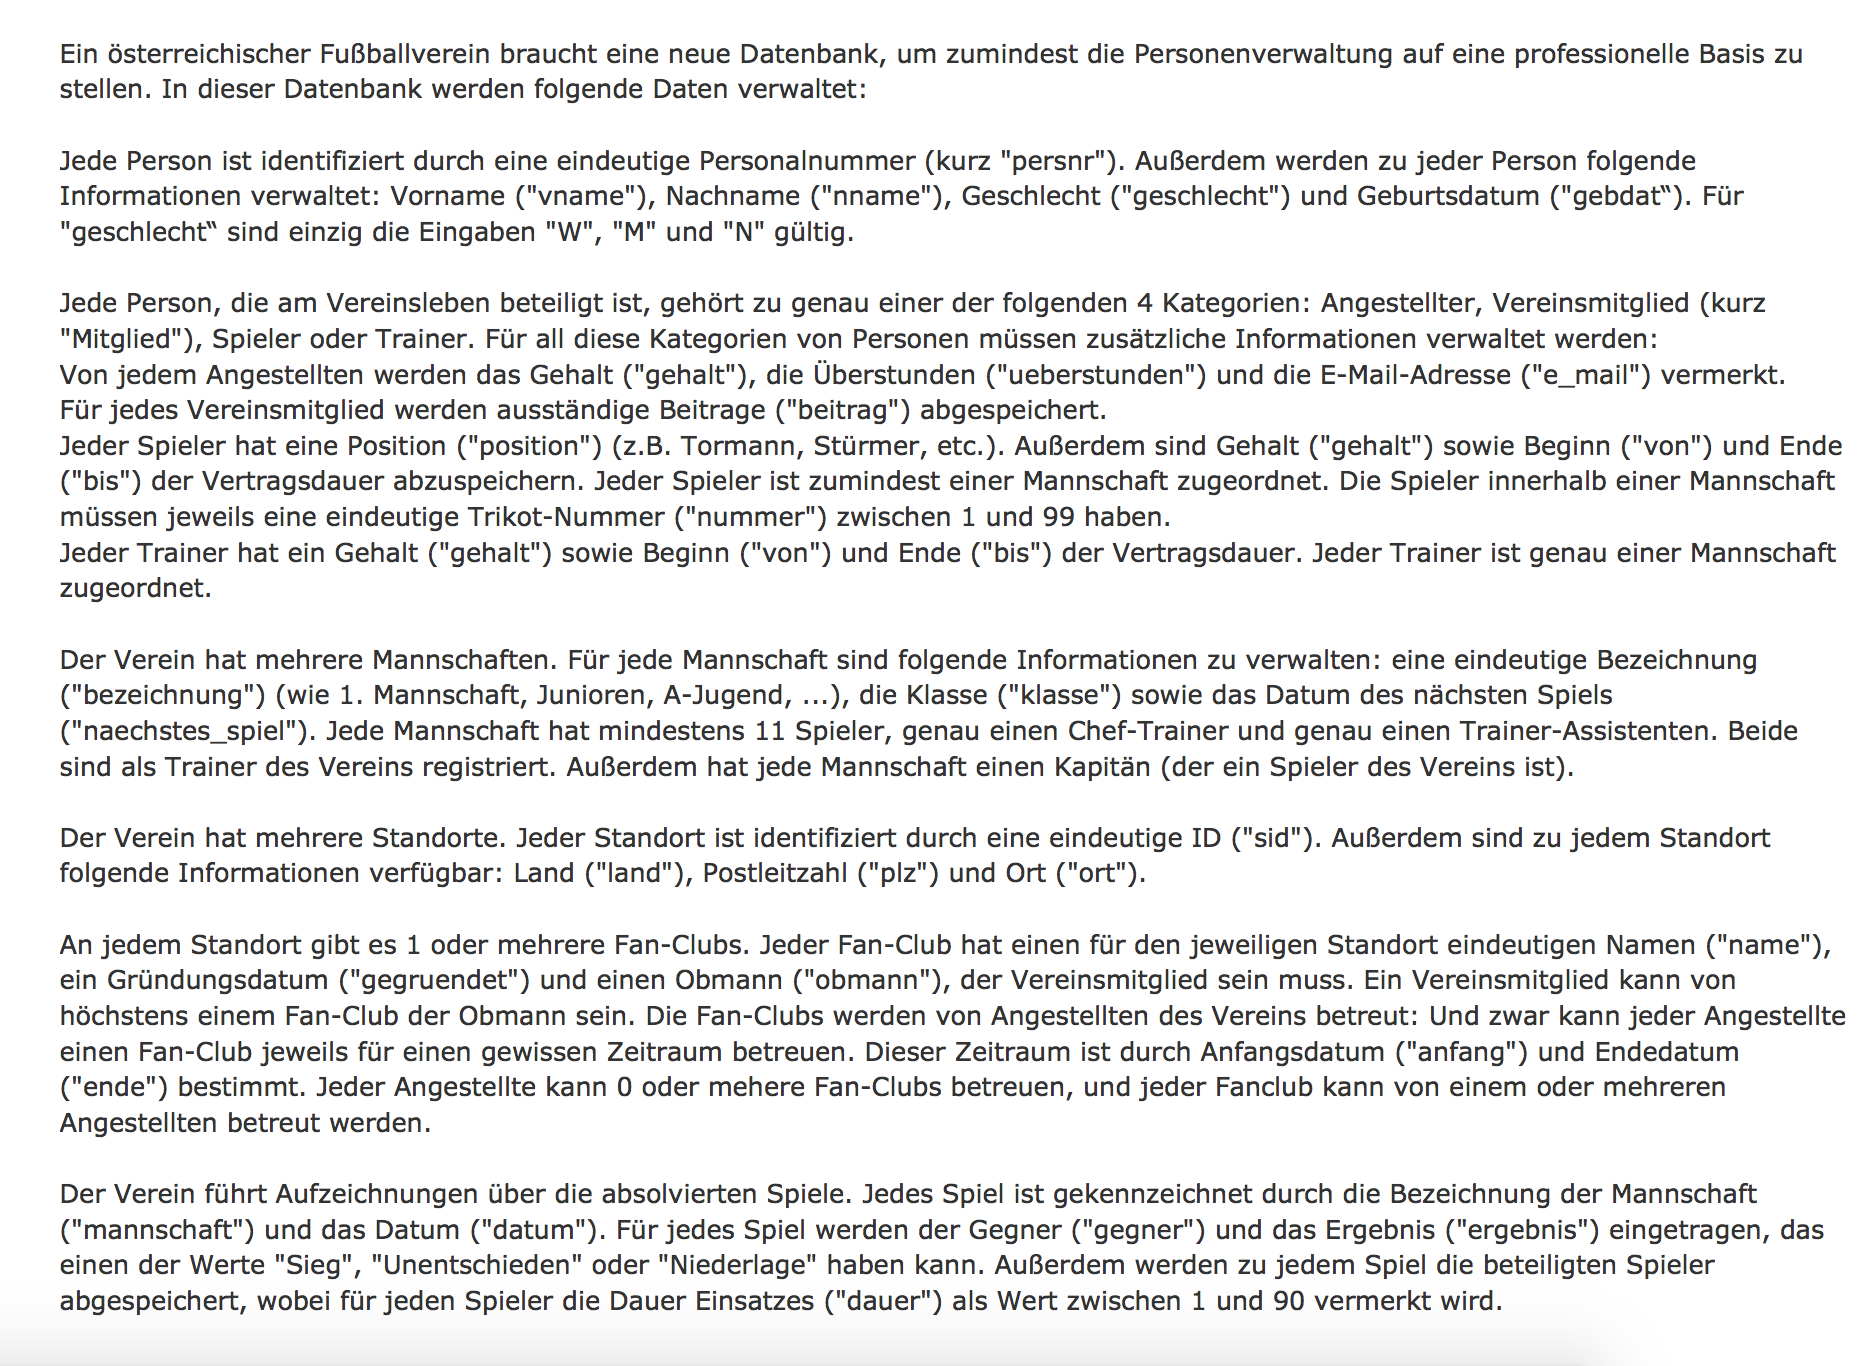
\includegraphics[scale=0.5]{images/angabe.png}

\section{Vorraussetzungen}
\subsection{Server starten}
\subsection{SSH - Verbindung}
\subsection{Postgres}
Datenbank, User erzeugen, Rechte verteilen \& Einloggen

\lstset{language=SQL}
\begin{lstlisting}
CREATE DATABASE verein;
CREATE USER manager WITH PASSWORD 'iderfrein';
GRANT ALL ON DATABASE verein TO manager;
\end{lstlisting}

Connection :
\lstset{language=bash}
\begin{lstlisting}
psql -d verein -h localhost -U manager -W
\end{lstlisting}
\section{Aufgaben}

\subsection{CREATE-Befehle}
Schreiben Sie die nötigen CREATE-Befehle, um die vorgestellten Relationen mittels SQL zu realisieren.
Dabei sind folgende Punkte zu beachten:

\subsubsection{Die Datenbank soll keine NULL-Werte enthalten.}
Dies lösst sich umsetzen, indem man am Ende des Attributes ein 'NOT NULL' anfögt.\newline
Beispiel:
\lstinputlisting[language=SQL, firstline=16, lastline=22]{../sql/create.sql}

\subsubsection{Realisieren Sie folgende Attribute mit fortlaufenden Nummern...}
...mit Hilfe von Sequences und Serial: "persnr" von Personen und ''sid'' von Standorten.
\begin{itemize}
\item För das ''persnr'' - Attribut sollen nur gerade, 5-stellige Zahlen vergeben werden (d.h.: 10000, 10002, ..., 99998).\newline

Sequences kann man sich wie eine Zöhlervariable vorstellen, welche im Hintergrund mitlöuft.
Erstellt wird unsere Sequence so :
\lstinputlisting[language=SQL, firstline=5, lastline=5]{../sql/create.sql}

Die 5 Stellen erhalten wir, indem wir uns an der Option \textbf{START WITH} bedienen.\newline
För die geraden Zahlen helfen wir uns mit einem Trick, in dem wir mit Hilfe von \textbf{INCREMET BY} immer um 2 erhöhen.\newline
=> da er nur immer um 2 erhöht, können nur gerade Zahlen kommen ! \newline

\item För das ''sid'' - Attribut sollen beliebige positive Zahlen (d.h. 1,2, ...) vergeben werden.\newline
Falls zwischen 2 Tabellen zyklische FOREIGN KEY Beziehungen herrschen,
dann sind diese FOREIGN KEYs auf eine Weise zu definieren, dass es möglich ist, immer weitere Datensötze mittels INSERT in diese Tabellen einzufögen.\newline
Die positiven Zahlen erhalten wir mittels einer \textbf{CHECK} - Constraint.\newline
\lstinputlisting[language=SQL, firstline=68, lastline=68]{../sql/create.sql}

\end{itemize}

\subsection{INSERT-Befehle}
Schreiben Sie INSERT-Befehle, um Testdaten för die kreierten Tabellen einzurichten. \newline
Jede Tabelle soll zumindest 10.0000 Zeilen enthalten. \newline
Sie dörfen die Wahl der Namen, Bezeichnungen, etc. so einfach wie möglich gestalten, d.h.: Sie mössen nicht "real existierende" Fuöballer-Namen, Lönder, Stödte, etc. wöhlen. \newline
Stattdessen können Sie ruhig 'Spieler 1', 'Spieler 2', 'Land 1', 'Land 2', 'Stadt 1', 'Stadt 2', etc. verwenden. \newline
Sie können för die Erstellung der Testdaten auch entsprechende Generatoren verwenden! \newline
\textbf{Nicht mein Kompetenzbereich, deshalb erstmal aufgeschoben.}

\subsection{DROP-Befehle}
Schreiben Sie die nötigen DROP-Befehle, um alle kreierten Datenbankobjekte wieder zu löschen.
z.B
\lstinputlisting[language=SQL, firstline=2, lastline=5]{../sql/drop.sql}
\clearpage

\section{Problemlösungen mittels SQL}
\lstinputlisting[language=SQL, firstline=1]{../sql/aufgaben.sql}

\section{Hier und dazwischen}
In diesem Kapitel möchte ich auf die Dinge eingehen, welche mich während meines Erarbeitens behindert haben.

\subsection{Das Upgrade auf Postgres 9.5}
Hört sich doch auch einfach an, oder?
Tja, falsch gedacht.
Naja zumindest halbwegs.
Nachdem ich mein Upgrade auf Postgres 9.5 machte, lief die Internet - Verbindung in meiner Virutal Machine einfach nicht mehr.
Er hat nichtmal die Netzwerkkarte angezeigt. Tote Maus.
Mit verkrampfter Maushand, welche sich über die letzten Tage entwickelte, wegen dem Kampf-Fehler-Googlen, müssen wir unser Debian-System backupen, und eine neue Distributation installieren.
Was ich dabei lernte :
\subsubsection{Backup machen mittels pg\_pgdumapll}
Um unsere Datenbank von Postgres zu sichern, nutzen wir entweder pg\_dump oder pg\_dumpall.
Ich nutzte pg\_dumpall, um gleich alle Datenbanken, Nutzer, etc. zu sichern.
\lstset{language=bash}
\begin{lstlisting}
pg_dumpall > verein.out
\end{lstlisting}
\subsubsection{aber wie übertrage ich jetzt die File ohne Netzwerkkarte?}
Der Ausweg bietet ein "Turnschuh"-Netzwerk. (USB - Verbindung)
Hierbei wiederhole ich mir meine alten Linux - Skills vorallem im Bereich mount.
Was ich interessant gefunden habe ist, dass bei mount -l nicht alle ungemounteten Datenträger angezeigt werden.
Wir mussten hierbei auf lsblk ausweichen.

\subsection{Das Upgrade auf El-Capitan}
Bis heute bereue ich meinen Kauf bei Apple meines Macbooks nicht.
Doch manchmal könnte ich wegen Apple dermaßen auszucken, und würde 
am Liebsten meinen Laptop aus dem Fenster werfen.
So musste ich um Qt installieren zu können,
XCode installieren, und um dies wiederum installieren zu können,
musste ich die Version meines Macs auf nächst-höheren Level bringen.
Zache G'schicht, ge'?
Aber das ist noch nicht alles !
Mein \LaTeX - Programm unter Mac kommt mit der neuen Version leider nicht zu Recht. So habe ich nun meine ganze \LaTeX - Arbeit (Protokoll) auf Debian umlagern müssen.
Leider habe ich mit diesem Vorgang viel Zeit verloren.

\subsection{Die Libary brauen?}
Meine Probleme hatte ich auch mit der Libary.
Tage lange gab mir Qt die Fehlermeldung '<pqxx/pqxx> not found' aus.
Nach längerem Seufzen und googeln wird meine Frust zu groß und ich breche meine Suche ab.
Auch Klassenkollegen können mir zu dem Problem nicht weiterhelfen.
Schlussendlich hilft mir Koll. Dolezal weiter, der mir erzählt, dass man die heruntergeladene Packages
erst brauen muss und intern installieren muss.

\lstset{language=bash}
\begin{lstlisting}
ruby -e "$(curl -fsSL https://raw.githubusercontent.com/Homebrew/install/master/install)" < /dev/null 2> /dev/null
brew install pqxx
\end{lstlisting}

Auwählen tue ich aber trotzdem bei Qt 'external libary'?
Keine Ahnung warum, aber bei 'internal libary' wurde diese nicht erkannt.

\subsection{Wäre doch zu schön, wenn nach dem Libary - Install alles funktionieren würde, oder?}
Nun wollte ich natürlich noch die Verbindung zu meiner VMWare herstellen.
Alle Eingaben waren richtig, und der Server war auch am Laufen.
Auch postgres lief.
Dies stellte ich mit Hilfe von folgendem Code fest.
\lstset{language=bash}
\begin{lstlisting}
netstat -tlpn
\end{lstlisting}
Ändern kann man den Port von Postgres übrigens unter:
\lstset{language=bash}
\begin{lstlisting}
vi /etc/postgresql/9.5/main/pg_hba.conf
\end{lstlisting}
Für den Restart von Postgresql:
\begin{lstlisting}
service restart postgresql
\end{lstlisting}

\newpage
\section{Plädoyer und Worte, die ich loswerden will...}
Auch wenn ich beim Projekt komplett neue Einblicke bekam, vorallem meine Linux --- Kenntnisse aufgefrischt habe, vorallem beim Helfen von Linux-Schwierigkeiten bei meinen Kollegen, und nicht zuletzt auch die Freude an \LaTeX  wiederendeckt habe, fand ich es schade, dass wir in der meisten Zeit komplett auf uns allein gestellt waren, und meist nur ein Hint zum Weiterarbeiten gegeben wird. Gerne nehmen sich die Lehrer auch für einen Zeit, ich schätze das auch sehr. Wirklich ! Aber sollten die Aufgaben so gestellt sein, dass ich dann den Lehrern wegen jeder 2. Unklarheit nachrennen muss? Ist das ein konstruktiver Unterrichtsstil?
Was hier stattfindet ist ganz einfach zu erklären:
\linebreak
\textbf{Leidenschaftliche Medientechniker werden zu Skriptkiddies und Systemtechnikern, wie Deutsche Militärkampfhunde umdressiert.}

\textbf{Das Verhältnis zwischen Medientechnik und Systemtechnik ist komplett unausgewogenen.}

Obwohl wir doppelt soviele Medientechnikstunden wie Systemtechnikstunden haben, spüre ich bei Medientechnik wenig. (gerade mal bei Schabasser macht mit uns regelmäßig Projekte)

Im Gegensatz dazu ist Systemtechnik viel spürbarer : 
Anstatt mich auf meine Leidenschaft Medientechnik fokussieren zu können, muss ich mich bis spät in die Nacht hinein damit herumschlagen, warum bei Qt meine Libary nicht gefunden wird.

Mit großer Frust und Nerven gehe ich dann zu Bett und blicke mit wahnsinniger Motivation in den nächsten Tag. Da kann man schon verstehn, warum wir kontinuierliche Zuspätkommer haben, oder Schulkollegen ... in die Schule kommen.
Nicht weil sie zu müde sind kommen sie zu spät, ganz einfach weil sie diese frustrierte Stimmung mit nach Hause nehmen und dann damit am nächsten Tag aufwachen.
Eigentlich schade. Ich war damals ja auch noch fasziniert von Pascal, Python und vorallem Linux, daher weiß ich was für ein Erfolgserlebnis man in der IT verspüren kann.
\textbf{Mit dieser Meinung vertrete ich zwar nicht die ganze Klasse, allerdings habe ich von einigen Zustimmung zu dem obrigen Absatz erhalten.}

\begin{quote}
	\textbf{'Vater, vergib ihnen, denn sie wissen nicht, was sie tun.'}\linebreak
	- Lukas, Kapitel 23, Verse 34
\end{quote}

Und es ist ja nicht so, als ob wir faul wären. Es ist einfach so, dass uns durch diese überforderlichen Aufgaben die Interesse und der Spaß an der Ausbildung vergangen ist.
Was bringt es, diese Leute zu den besten ITlern bzw. Systemtechnikern zu machen, wenn dass nacher sowieso niemand mehr beruflich machen will, weil die Freude an der Sache vergangen ist.